\documentclass[12pt, a4paper]{article}
\usepackage{amsmath}
\usepackage{amsfonts}
\usepackage{amsthm}
\usepackage{mathtools}
\newtheorem{theorem}{Theorem}[section]
\newtheorem{definition}{Definition}[section]
\numberwithin{equation}{section}
\usepackage{pgfplots}
\pgfplotsset{width=10cm,compat=1.9}
\graphicspath{ {img/} }
\DeclareGraphicsExtensions{.png, .jpg}

\title{Machine learning strategies}
\author{Kristian Wichmann}

\begin{document}
\maketitle

\section{Introduction}
This note describes a number of strategies, tips and tricks for successfully navigating actual machine learning projects.

\subsection{The project development cycle}

\begin{figure}
\centering
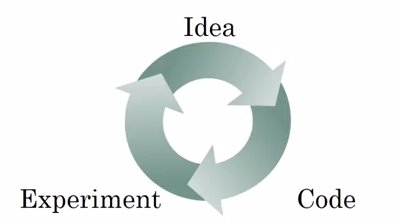
\includegraphics[width = 0.5\textwidth]{dev_cycle}
\caption{The project development cycle}
\label{fig:cycle}
\end{figure}

Basically, the evolution of a ML project over time comes in cycles of three phases:
\begin{equation}
\textrm{Idea}\rightarrow\textrm{Code}\rightarrow\textrm{Experiment}
\end{equation}

In short: Start with an idea, implement it in code. Then get your hands dirty and experiment with running the code in different ways. Eventually, this will hopefully lead to getting a new and hopefully better idea, which will start the cycle over again, until a satisfactory product has been build.

It is generally adviced to get started relatively fast: Get an initial - even if simple - idea, and implement the code as soon as possible. This is preferable to wasting too much time pondering the details of the problem instead of actually getting started with the project development. 

Build you first system quickly, then iterate. The material below should help you do this effectively.

\subsection{Orthogonalization}
\textit{Orthogonalization} is essentially knowing what to tune to achieve what effect.

Ideally, when turning one "knob" on you ML problem, it should only affect one aspect of the outcome - each does only one, easily interpretable, thing. That way, you may tune one "knob" at a time to get the desired behaviour from the algorithm.

\subsubsection{Chain of assumptions}
When building an ML product, there's a chain of assumptions being made:
\begin{itemize}
\item We can fit the parameters well to the training set, so that the chosen cost function is low. In other words, we assume that we can get an acceptable performance on the training set. Sometimes this means getting human level performance or better.
\item We then hope this model also does well on the dev set. Failure to do so us typically a sign of overfitting.
\item And on the test set as well.
\item This should lead to good performance out in the real world.
\end{itemize}
For each of these problems, we have different "knobs" to turn in order to get the desired result. Here's some examples that may help achieve succes for each:
\begin{itemize}
\item Performance on the training set:
	\begin{itemize}
	\item Training a bigger network, or more generally a model with greater capacity.
	\item Choosing a better strategy for gradient descent. ADAM for instance.
	\item Train your model for more epochs.
	\end{itemize}
\item Performance on the dev set:
	\begin{itemize}
	\item Regularization, like ridge regression or dropout.
	\item Getting a bigger training set.
	\end{itemize}
\item Performance on the test set:
	\begin{itemize}
	\item Get a bigger dev set.
	\end{itemize}
\item Performance in the real world:
	\begin{itemize}
	\item Change the dev set to better correspond to real world data.
	\item Change the cost function to better fit the problem.
	\end{itemize}
\end{itemize}
We'll dive into a lot of these in more detail below.

\subsubsection{Non-orthogonal example: Early stopping}
Some strategies are non-orthogonal. I.e. they affect several of the points in the chain above at the same time. One such example is early stopping, where performance is monitored on the training and dev set simultaneously. Therefore, in this case we're "tuning two knobs" at once.

\section{Setting your goal}
This is the crucial question for training the model: What are our optimization criteria? Which quantities do we want to optimize, and under which contraints (if any)? This section outlines a number of strategies, and thoughts on when/if it's a good idea to change these goals along the way.

\subsection{Single evaluation metric}
In this case, there's simply one quantity which gauges the performance of the model. We can then train the model to optimize the quantity. The cost function is an example.

If we have a number of discrete options to choose from, we can simply pick the one with the highest/lowest performance.

Often, there will be several relevant metrics related to a problem. Sometimes we can combine these into one, as the following example shows.

\subsubsection{Example: $F_1$ score}
For classification, both precision and recall are relevant metrics to consider. If we have trained two classifiers A and B with the properties when evaluated on the dev set shown in table \ref{table:two_classifiers}, it is not immediately clear which one we should pick; there's often a trade-off between the two.

\begin{table}
\centering
\label{table:two_classifiers}
\begin{tabular}{l|c|c|}
\cline{2-3}
                                   & \multicolumn{1}{l|}{Precision} & \multicolumn{1}{l|}{Recall} \\ \hline
\multicolumn{1}{|l|}{Classifier A} & 95\%                           & 90\%                        \\ \hline
\multicolumn{1}{|l|}{Classifier B} & 98\%                           & 85\%                        \\ \hline
\end{tabular}
\caption{Properties of two classifiers}
\end{table}

One way to combine the two, is the $F_1$ score, which is the harmonic mean of the precision ($P$) and recall ($R$):
\begin{equation}
F_1=\frac{2}{\frac{1}{P}+\frac{1}{R}}=\frac{2}{\frac{P+R}{PR}}=\frac{2PR}{P+R}
\end{equation}
We may now calculate the $F_1$ score of the two classifiers:
\begin{equation}
A: F_1=\frac{2\cdot 0.96\cdot 0.90}{0.96+0.90}\approx 92.4\%\quad
B: F_1=\frac{2\cdot 0.98\cdot 0.85}{0.98+0.85}\approx 91.0\%
\end{equation}
So, with $F_1$ score as the single evaluation metric, we should pick classifier A.

\subsection{Satificing and optimizing metrics}
Often, it is not possible to include all the relevant metrics into one. We can get around this problem by deciding on a metric that we want to optimize, and for the others decide on a performance that is good enough. The latter as known as satificing metrics.

\subsubsection{Example: Image classification}
We have trained three image classifiers, and their accuracies on the dev set as well as run time is shown in table \ref{table:satisficing}. We want to optimize accuracy with run time as a saticficing metric, so that is should be below 100 ms.

\begin{table}
\centering
\label{table:satisficing}
\begin{tabular}{l|c|c|}
\cline{2-3}
                                   & \multicolumn{1}{l|}{Accuracy} & \multicolumn{1}{l|}{Time/ms} \\ \hline
\multicolumn{1}{|l|}{Classifier A} & 90\%                           & 80                        \\ \hline
\multicolumn{1}{|l|}{Classifier B} & 92\%                           & 95                        \\ \hline
\multicolumn{1}{|l|}{Classifier C} & 95\%                           & 1500                        \\ \hline
\end{tabular}
\caption{Three image classifiers}
\end{table}

The satisficing condition disqualifies classifier C, even though it has the highest accuracy. Of the two that are left, classifier B is picked, as it has the highest accuracy.

\subsection{Distributions of dev vs. test sets}
In a sense, out goal is set by choosing the metric/loss function along with the dev set. Together, these can be thought of as a dart board target. Through the idea $\rightarrow$ code $\rightarrow$ experiment cycle, an ML project team can get progressively closer to hitting the bullseye of this dart board.

But when the time comes to checking the performance at the test set, we might be in trouble if we have not chosen it from the same distribution as the dev set! If these differ, we have actually "moved the target" for the test set, and hence the performance will suffer.

\subsubsection{Example: Geographical differences}
Let's say our data are divided into geographical regions: North America, South America, Europe, Asia, Africa, Australia. Now, imagine we choose our dev and test sets as follows:
\begin{itemize}
\item Dev set: North America, South America, Europe
\item Test set: Asia, Africa, Australia
\end{itemize}
Here, we would be in trouble, since these represents to "different targets" (two different distributions): Good performance on the dev set, may not correspond to good performance on the test set!

Instead, all of the data should be shuffled, and randomly distributed between the dev and test sets. Then the two sets come from the same distribution.

\subsubsection{Size of train, dev and test sets}
Earlier, it might have been adviced to have a split in size between the three sets be 60\% training set, 20\% dev set, and 20\% test set (or figures around these lines).

However, in the big data era, we often have a so much data, that there's no reason to make the dev and test percentages so large.

The test set should be large enough, that it ensures confidence in the performance of the model. The dev set should be of comparable size. Exact measures depend on the problem, but if, for instance we have a million data points, 1\% is 10000 samples! Often, this will be enough for confidence in the model. So, a reasonable split for such modern data sets is often closer to 98\% training set, 1\% dev set, and 1\% test set.

Sometimes, you may even forego having a test set, and simply work with a dev set (which confusingly, is then sometimes referred to as the test set). This is generally not recommendable, but may work nonetheless.

\subsection{When to change metrics and/or dev/test sets}
Sometimes, we find that the target we have set is simply not appropriate for what we wish to achieve. This section offers some insight into detecting such a problem, and how to deal with it.

\subsubsection{Example: Cat image classifier}
Let's say, you're building a cat app, and have made two binary classifiers for distringuishing between cat and non-cat pictures. You have chosen the - appearantly perfectly reasonable - optimization metric to be classification accuracy.

Now, on the dev set classifier A has an accuracy of 3\%, while classifier B has 5\%. So initially classifier A is chosen. However, it turns out, that classifier A lets some pornographic images through! This is of course unacceptable for a cat app.

We are now in a situation, where the "target" set (i.e. the metric and dev set) prefers classifier A, while you/the app users prefer classifier B. This is a sign that it's time to move the "target"!

\subsubsection{Changing the metric}
In the example above, we might choose to penalize the mis-classified pornographic images much heavier than other errors. Let's see how. The original metric to be minimized is:
\begin{equation}
\frac{1}{m}\sum_{i=1}^m\delta_i
\end{equation}
Here $m$ is the number of samples in the dev set, and $\delta_i$ is either 0 or 1, depending on whether or not the sample is mis-classified or not.

Now, we introduce a weighting factor $w_i$, depending on whether or not the image is pornographic in character:
\begin{equation}
\label{new_metric1}
\frac{1}{m}\sum_{i=1}^m w_i\delta_i
\end{equation}
Here, we set $w_i$ equal to 1 for most images, and a larger number, like 10 or maybe even 100, for pornographic ones. Finally, we may wish to change the normalization constant, so we get a rating between 0 and 1:
\begin{equation}
\label{new_metric2}
\frac{1}{\sum_{i=1}^m w_i}\sum_{i=1}^m w_i\delta_i
\end{equation}

Note the orthogonalization in this approach: First, we worry about changing the metric to something more appropriate. Then we go through development cycles to improve performance with regards to the new metric.

\subsubsection{Another example: More cat images}
Consider the same cat image classifier example as above. However, in this case, the problem is, that the images we've used for the dev/test sets are images collected on the internet. These are often taken by professional photographers, and so tend to be of much higher quality/clarity than ones taken by amateaurs, who are the typical users of the cat app.

So when deployed, the classifier actually does much worse than it did on the dev/test sets, since the real app images comes from a different distribution.

This would be a good time to change the dev/test sets (and maybe the metrics) to better fit the actual problem.

\section{Comparison to human-level performance}

\subsection{Bayes error rate}
The Bayes error rate (or Bayes optimal error) for a machine learning problem, is the theoretical lower bound of how well an algorithm is able to perform. This rate is usually not zero, as the quality of the data may not be sufficient to make a perfectly performant algorithm.

\subsection{Avoidable bias}
We are interested in estimating the Bayes error rate, since any algoritm we make will have an error rate higher than the Bayes error rate. The difference between Bayes error rate and actual rate shows how much room we have for improvement. This is known as the avoidable bias.

\subsection{Human level performance as a proxy for Bayes error rate}
Human level performance can mean many things. If we want to diagnose a patient based on x-ray images, the average human will not do too well. A trained doctor will do much better. And a team of trained doctors even better.

What all these have in common is, that since they are algorithms, their error rate must me at least as large as the Bayes error rate of the problem! Therefore, if we know the human error rate (or the best one if we have several, as in the example above), we have a limit on the Bayes error rate, and therefore also on the avoiadable bias.

\subsection{Beyond human level performance}
There is however no guarantee that human level actually is the Bayes error rate, though for some tasks it will be close. But often, it is possible to develop an algoritm that will have a lower error rate than the best human performance. However, in this region, it is trickier to guide the development. The reason is, that as long as the algoritm performs worse than humans, we have the following advantages when developing:
\begin{itemize}
\item We can get more data labelled by human with relative ease.
\item We can gain insights from manual error analysis: "Why did a person get this right?"
\item We can do a better analysis of bias and variance (see below).
\end{itemize}

\subsection{What to focus on? Bias or variance?}
Let's consider a task, for which our algorithm has an error rate of 8\% on the training set and 10\% on the dev set. The question is now, if we should focus our energy on correcting bias (lowering error on training set) or variance (lowering error on dev set).

If we know what the human level performance is, we can use it as a proxy for the Bayes error rate. This will be helpful in guiding this decision.

If the human error level is 1\%, then our algorithm, isn't really doing a terribly good job on the training set: We know that the avoidable bias is at least 7\%, while the correponding variance (the different between training and dev set errors) is 2\%. Here, it would make sense to work on increasing the capacity of the algorithm. I.e. work on reducing bias.

On the other hand, if the human error level var 7.5\%, then chances are, that our algorithm is actually doing pretty well (unless we have reasons to suspect the Bayes error rate is drastically lower than human performance). Here, working to reduce variance, for instance by regularization or gathering more data, would make sense.

\subsubsection{Summary}
As long as human error is a reasonable proxy for the Bayes error, it makes sense to make a decision based on comparing the following:
\begin{itemize}
\item The avoidable bias: The difference between (the best) human-level error and training set error.
\item Variance: The difference between training set error and dev set error.
\end{itemize}

\subsection{Beyond human-level performance}
Here, making an informed decision as in the previous section is much harder: We can no longer use human-level error as a proxy for Bayes error, and hence, we are much more in the dark.

That does not mean that further improvements are not possible, but there's fewer clues to what might be an effective strategy.

\section{Case study: Bird recognition}
Let's play a game: You are the top machine learning researcher in a city where people are afraid of birds. You are therefore put in charge of developing an image classifier that detects birds in pictures.

To this end, you're given a labelled set of 10,000,000 security camera pictures, where each picture is classified as having a bird in it ($y=1$) or not ($y=0$).

\subsection{Choice of metric}
The City Council tells that they want an algorithm which has the following properties:
\begin{itemize}
\item Has high accuracy.
\item Runs quickly and takes only a short time to classify a new image.
\item Can fit in a small amount of memory, so that it can run in a small processor that the city will attach to many different security cameras.
\end{itemize}
Since having three separate metrics complicates your work, making it hard to make a fast decision between potential classifiers, you and the council decide on a satisicing metric scheme as follows:
\begin{itemize}
\item Accuracy as the optization metric.
\item Classification time as a satisficing metric: The classification should take at most 10 seconds.
\item Memory usage as a satificing metric: The model should fit within 10 MB of memory.
\end{itemize}

\subsection{Division into training/dev/test sets}
Since there's a large amount of data, there's no reason to make the dev and test sets very large, percentage-wise. You judge that testing on 250,000 images should be enough to ensure confidence in a model. Therefore, you randomly split the data as follows:
\begin{itemize}
\item Training set: 9,500,000 images.
\item Dev set: 250,000 images.
\item Test set: 250,000 images.
\end{itemize}

\subsubsection{Getting additional data}
After doing this, you are informed, that the City Council has acquired an additional 1,000,000 labelled images from concerned citizens worried about the bird threat.

These images overall does not have the same clarity and resolution as the ones from the security cameras: They have a different distribution.

Since the final classifier will actually use security camera footage, adding these to the test set is a bad idea. So is adding them to the dev set, as the dev and test set should come from the same distribution. However, there is no major problem in adding them to the training set, since the algorithm will be tuned to perform will on the dev set anyway.

\subsection{Bias/variance considerations}
You train a first iteration of the model, and it turns out that is has the following error rates:
\begin{itemize}
\item Training set error: 4\%.
\item Dev set error: 4.5\%.
\end{itemize}
This makes the variance 0.5\%, but initially your only estimate of the avoidable bias is, that it is 4\% or less.

To getter a better idea, you look to human-level performance on the classification task. It turns out, that most people have an error rate around 1\%. However you also find that trained ornitologists have an error rate of 0.3\%. However, a team of ornithologists does even better, having an error rate of 0.1\%!

Hence, your best estimate of the human-level performance error rate as a proxy for Bayes error is 0.1\% - the lowest score any human, or team of humans, you tested achieved.

With this in mind, you see that the avoidable bias is at least 3.9\%. Much more than the variance of 0.5\%. You conclude that you best course of action for the next development cycle is to focus on reducing the bias. Some strategies could be easing regularization of the model, or rebuilding a model with greater capacity.

\subsection{Test set performance}
The next iteration of you algorithm, which you also run on the test set, has the following error rates:
\begin{itemize}
\item Training set error: 2\%.
\item Dev set error: 2.1\%.
\item Test set error: 7\%.
\end{itemize}
We see that the dev training and dev sets have almost the same error rate, so it has been fit well to the dev set. However, the jump in error for the test set shows that it has indeed overfit the data to the dev set!

To remedy this, we could augment the size of the dev set.

\subsection{Beyond human-level performance}
After working hard on improving the algoritm for some time, you end up with a classifier with the following performance:
\begin{itemize}
\item Human-level error: 0.10\% (as before)
\item Training set error: 0.05\%.
\item Dev set error: 0.05\%.
\end{itemize}
Since the algorithm is now better than human-level performance, we can no longer use the 0.10\% as a proxy for Bayes error. Indeed, we see that the Bayes error must now be less than or equal to 0.05\% While there still may be room for further improvements, such developments will be slow, since we no longer have an estimate of avoidable bias.

\subsection{Moving the "target"}

\subsubsection{Competition!}
You find out, that the City Council has hired one of your competitors to work on the problem as well. And it turns out that even though your model has a higher accuracy, the council likes your competitor's model better, as it has fewer false positives, leading to fewer false bird alarms.

To remedy this situation, you find that it's time to change your optimization metric, introducing a large penalization weight for false positive classifications as shown in equations \ref{new_metric1} and \ref{new_metric2}.

\subsubsection{New bird species}
Subsequent development gives you back the edge over the opposition, but now you are faced with a new problem: A new bird species is being sighted, and your classifier's performance slowly drops as a result of this new distribution of the real images. You are given a few months to remedy this situation, but you only have 1000 images with the these animals in them to work with.

So, since the algorithm still does rather well at recognizing birds in general, you decide that it's not much use to add any of the 1000 images to the training set. Instead you add 500 to each of the dev and test sets, and introduce another penalization weight for misclassifications of these images, hence moving the "target" to a position of special interest in getting these pictures right.

\subsection{Incorporating existing data}
The City Council has found, that in addition to your classifier, having cats in the city also helps reduce the number of bird sightings. Having previously worked with cat images, you have a large back catalogue of labelled cat/non-cat images. 100,000,000 images, in fact! Training a model on this massive data set takes about two weeks.

You decide that starting by training a model on a much smaller data set, like 1,000,000 images is worth the advantage of a getting a quick start, even if the initial model may be sub-optimal. Getting faster computers from the council would also greatly improve the speed of your progress.


\section{Error analysis}
Let's go back to out favorite example: The binary cat image classifier. Suppose you have an error rate of 10\%, and someone from the team suggests, that a lot the errors are dog images being classified as being cat images. The question now is whether it is worth the time and energy to focus specifically on this problem.

\subsection{Manual error checking}
To do so, it is suggested that you take a random sample of, say, 100 of the misclassified pictures. Then go through them by hand, and count how many of the errors are actually dogs classified as cats. Then that number can be used to estimate the best-case improvement that might results from fixing the problem.

If, for instance, that 5 of the 100 pictures were dog mistaken for cats, then 5\% of the 10\% errors, i.e. 0.5\%, is an estimate of how much the error rate could improve from this particular focus. This is also known as a ceiling - remember that it's a best-case scenario. Whether this is worth your effort will of course depend on the problem.

If, on the other hand, there was 50 out of 100 images with this problem, the ceiling would be 5\%. In this case, it is almost certainly a good place to concentrate efforts.

No matter what the ceiling value turns out to be, this is a procedure that will not take you many minutes, but will potentially save you lots of the frustration that may come from wasting resources on insignificant improvements.

\subsubsection{Testing several hypotheses}
If there's several ideas on the board for what may cause errors, you can check for several at the same time while going though your image sample. The observations can be summarized in a simple table/spreadsheets; Causes of errors as columns, and individual images as rows. Make a tag if the error is due to the relevat column.

Be sure to leave a column open for comments, so you can jot down anything unusual during the inspection. You might just stumble upon a new hypothesis by reviewing those! Also, leave a column for incorrectly labelled data (see next section).

When done, you can the sum up each column, and calculate ceiling values from those.

\subsection{Incorrectly labelled data}
As you go through a sample of images as described above, you may run into incorrectly labelled images. It is almost inevitable that there will be some mislabelled data, especially in a large data set, but depending on the amount and character of such wrong labels, we may have a problem.

\subsubsection{Training set}
Typically, training sets are large, and so tend to be rather robust with respect to a few, randomly mislabelled data. Since we usually make sure that the algorithm will not overfit, a few weird data points tend not to skew the overall picture.

However, if these errors are not random, i.e. if the mislabelling happens according to some kind of system, the training set will be biased. ML algorithms are very good at picking up any kind of systematic in the data, and hence we could have a big problem.

\subsubsection{Dev set}
This is the error you can estimate by manually going through the images. Again, you can use this to estimate a ceiling value to decide whether going through the labels of the dev set would be worth your time.

If you are comparing different classifiers, this will also give you a margin, within which it will not make sense to make such a comparison. For instance if the "misclassification ceiling" is 0.6\%, it makes little sense to claim that a classifier with an error rate of 2.1\% is better than one with an error of 2.6\% - as the difference is smaller than 0.6\%!

\subsection{Correcting labels}
Let's assume that you've decided it's worth the effort to correct the labelling of your data. Which sets to correct?

As noted above, unless there's known biases in your training set, there's usually no reason to go through the (usually huge) training set.

But the dev and test sets should both be corrected. Otherwise, the distributions will not remain the same.

\subsubsection{Errors vs. non-errors}
Usually, there will be data point the algorithm gets wrong than right. It's natural to focus on the errors, but it might be a good idea to at least sample some of the non-errors to see if there's similar problems happening there too.

\section{Mismatched training/dev/test sets}
Sometimes, the distribution of the training set and the dev/train sets are not the same. For instance, if we'd done the label correction mentioned above, we would be in this situation. Another way this could happen is described in the example below:

\subsection{Example: Cat app (again)}
As noted earlier, if we want to train a cat image classifier for a cat app, it will be relatively easy to find a lot of cat images on the net. But such images will tend to be of high quality, and thus not from the same distribution as the ones the app will actually deal with.

Let's say that we have found/downloaded/scraped 200,000 high quality cat images from the web. We also have 10,000 more realistic images from a pre-test of the cat app. Clearly these numbers are skewed.

If we just shuffle all of the images and divide into train/dev/test sets, we are in trouble: We will set the wrong target, as most of the images from the dev/test sets are actually not reflective of the real image data the app will handle!

Instead, since our target is the pre-test app data, let \emph{all} of the dev/test sets be from this group! Let the dev set be the downloaded image and the rest of the app data. For instance, we might use the following split:
\begin{itemize}
\item Training set: All 200,000 web images, 5,000 app images.
\item Dev set: 2,500 app images.
\item Test set: 2,500 app images.
\end{itemize} 

\subsection{Bias and variance for mismatched sets}
So for one reason or the other, we may find ourselves in the situation where the training set and the dev/test sets come from different distributions. This may not be as big a problem as one might think. Let's take a look.

Let's consider the cat app again, and for simplicity let's assume the Bayes error is zero. After building a classifier, we get the following error rates:
\begin{itemize}
\item Training error: 1\%.
\item Dev error: 10\%.
\end{itemize}
Now conventionally, we would say that the avoidable bias is 1\%, and the variance is 9\%, indicating a clear overfitting problem. But, since we have different distributions for the two sets, it is only natural that the classifier has a hard time on the dev set. The question is how we may make decisions on how to proceed in this situation.

\subsubsection{The training-dev set}
One solution is to further subdivide the training set into two parts: The (proper) training set, and the training-dev set. These should be randomized, and hence will come from the same distribution. The training-dev set should be of a size comparable to the dev and test sets. So for instance, in the example above, a reasonable split would be:
\begin{itemize}
\item (Proper) training set: 202,500 randomly chosen images from (200,000 web images, 5,000 app images).
\item Training-dev set: The remaining 2,500 images from (200,000 web images, 5,000 app images).
\item Dev set: 2,500 app images.
\item Test set: 2,500 app images.
\end{itemize} 

\subsubsection{Mismatch error}
We can now look at the algorithms performance on the training-dev set along with the other three sets (and the Bayes error).

For instance, we might get the following:
\begin{itemize}
\item Training error: 1\%.
\item Training-dev error: 9\%.
\item Dev error: 10\%.
\end{itemize}
Here, we see that the variance is actually 8\%. The difference between the trainin-dev and dev errors - known as the mismatch error - is actually only 1\%. So the problem is overfitting rather than differences in distribution.

On the other hand we could have gotten the following:
\begin{itemize}
\item Training error: 1\%.
\item Training-dev error: 1.5\%.
\item Dev error: 10\%.
\end{itemize}
Here, the variance is 0.5\%, while the mismatch error is 8.5\%. Clearly, distribution difference is a much bigger problem.

Of course, we might also still have a bias problem if the training error is high compared to the (estimated) Bayes error. All of these cases are summarized in the next section.

\subsection{Summary: Errors and diagnostics}

\begin{table}[b]
\centering
\label{table:diagnostic}
\begin{tabular}{cc}
Bayes error (or proxy) &                           \\
$\downarrow$           & Avoidable bias            \\
Training error         &                           \\
$\downarrow$           & Variance                  \\
Training-dev error     &                           \\
$\downarrow$           & Data mismatch             \\
Dev error              &                           \\
$\downarrow$           & Dev set overfitting       \\
Test error             &                          
\end{tabular}
\caption{Errors and diagnostics in ML problem}
\end{table}

To summarize, we now have five relevant error rates as seen in table \ref{table:diagnostic}. The gaps between them and what they signify is also shown.

Do note, that sometimes dev error may actually be \emph{lower} than training-dev error. This can happen if the dev/test data are actually easier to classify.

\subsection{What to do about data mismatch?}
There's no standard solution to these kinds of problems, but nevertheless, this section contains some suggestions that might be helpful.

Is there a way to get more data similar to the dev set? Expanding the training set this way is the most obvious way to remedy the situation.

Manually compare samples from the training and dev sets. Try to get an idea of the differences. Consider how you can make the training set more similar to the dev set. If the dev set has blurred images, you might want to similarly distort images from the trianing set. OR if the dev set has noisy sounds, you might want to similarly add noise to your training set. Or you might synthesize similar data. Just beware that these alterations/new data do not follow patterns the learning algorithm may pick up on, as this can lead to overfitting.



\section{Learning from multiple tasks}


\section{End-to-end deep learning}


\section{Case study: Image recognition for driverless car}

\end{document}